% !TEX encoding = IsoLatin

% La riga soprastante serve per configurare gli editor TeXShop, TeXWorks
% e TeXstudio per gestire questo file con la codifica IsoLatin o Latin 1
% o ISO 8859-1.

% per commentare una riga mettere % al suo inizio
% per s-commentare una riga (ossia attivarla) togliere il % al suo inizio
%
\documentclass[pdfa% formato PDF/A, obbligatorio per l'archiviazione delle tesi di Polito
%,cucitura%lascia margine per la rilegatura
,twoside% per stampa fronte-retro (fortemente consigliato per tesi voluminose, opzionale per le altre)
,12pt% font pi? grande (12pt) rispetto a quello normalmente usato (11pt)
]{toptesi}
%
\usepackage{hyperref}
\hypersetup{%
    pdfpagemode={UseOutlines},
    bookmarksopen,
    pdfstartview={FitH},
    colorlinks,
    linkcolor={blue},
    citecolor={red},
    urlcolor={blue}
  }
% \documentclass[11pt,twoside,oldstyle,autoretitolo,classica,greek]{toptesi}
% \usepackage[or]{teubner}
%%%%%%%%%%%%%%%%%%%%%%%%%%%%%%%%%%%%%%%%%%%%%%%%%%%%
%
% Esempio di composizione di tesi di laurea.
%
% Questo esempio e' stato preparato inizialmente 13-marzo-1989
% e poi e' stato modificato via via che TOPtesi andava
% arricchendosi di altre possibilita'.
%
% Nel seguito laurea "quinquennale" sta anche per "specialistica" o "magistrale"

% Cambiare encoding a piacere; oppure non caricare nessun encoding se si usano
% solo caratteri a 7 bit (ASCII) nei file d'entrata.
%
\usepackage[latin1]{inputenc}% IMPORTANTE! usare codifica ISO-8859-1 per le lettere accentate
% \usepackage[outputdir=out,cache=false]{minted}

% !TEX encoding = IsoLatin

% per inserire uno spazio "fantasma" nella definizione di un'abbreviazione
\usepackage{xspace}

% per inserire un DOI senza problemi coi caratteri "strani" ivi presenti
\usepackage{doi}
\renewcommand{\doitext}{DOI }% originally was "doi:"

% per inserire correttamente le unit� di misura SI (incluse quelle binarie)
\usepackage[binary-units]{siunitx}
% se si desidera usare / invece che la potenza -1 per indicare "al secondo"
\sisetup{per-mode=symbol}

% per inserire codice di programmazione complesso
\usepackage{listings}% per inserire codice di programmazione complesso
\lstset{
basicstyle=\ttfamily,
columns=fullflexible,
xleftmargin=3ex,
breaklines,
breakatwhitespace,
escapechar=`
}

% modify some page parameters
\setlength{\parskip}{\medskipamount}

% riga orizzontale
\newcommand{\HRule}{\rule{\linewidth}{0.2mm}}
% esempio di creazione di semplici abbreviazioni
\newcommand{\ltx}{\LaTeX\xspace}
\newcommand{\txw}{TeXworks\xspace}
\newcommand{\mik}{MikTex\xspace}
\newcommand{\html}{HTML\xspace}
\newcommand{\xhtml}{XHTML\xspace}

% esempio di creazione di un'abbreviazione con un parametro (il cui uso � indicato da #1)
\newcommand{\cmd}[1]{\texttt{#1}\xspace}
% per citare un RFC, es. \rfc{822}
\newcommand{\rfc}[1]{RFC-#1\xspace}
% per citare un file (es. \file{autoexec.bat}) o una URI fittizia (es. \file{http://www.lioy.it/})
% per le URI vere usare \url o \href
\newcommand{\file}[1]{\texttt{#1}\xspace}
% per inserire codice di esempio in-line
\newcommand{\code}[1]{\lstinline|#1|}
% importante per i pathname Windows perch� non si pu� usare \ essendo un carattere riservato di Latex
\newcommand{\bs}{\textbackslash}
% definizione di un termine: formattazione ed inserimento nell'indice
\newcommand{\tdef}[1]{\textit{#1}\index{#1}}
% meta-termine, usato tipicamente nelle definizioni dei tag
\newcommand{\meta}[1]{\textit{#1}}
% abbreviazioni in inglese
\newcommand{\ie}{i.e.\xspace}
\newcommand{\eg}{e.g.\xspace}
\usepackage{cryptocode}
\usepackage{listings}
\usepackage{svg}
% modificare il path di inkscape nel caso di errori
\setsvg{inkscape={"C:/Program Files/Inkscape/bin/inkscape.com"}}
\svgpath{{chapters/images}}

\usepackage{xcolor}
\lstdefinestyle{json}{
  string=[s]{"}{"},
  stringstyle=\color{blue},
  comment=[l]{:},
  commentstyle=\color{black},
}
\begin{document}
\selectlanguage{english}


\ateneo{Politecnico di Torino}

%%% scegliere la propria facolt? (solo PRIMA dell'AA 2012-2013)
%
%\facolta[III]{Ingegneria dell'Informazione}
%\facolta[IV]{Organizzazione d'Impresa\\e Ingegneria Gestionale}
%\Materia{Remote sensing}% uso sconsigliato

%\monografia{Gestione informatizzata di un magazzino ricambi}% per la laurea triennale
\titolo{Self-Sovereign-Identity as a Service}% per la laurea quinquennale e il dottorato
\sottotitolo{Trusted Computation Offloading for IoT constrained devices}% NON obbligatorio, per la laurea quinquennale e il dottorato

%%% scegliere il proprio corso
%
%\corsodilaurea{Ingegneria dell'Organizzazione d'Impresa}% per la laurea di primo e secondo livello
%\corsodilaurea{Ingegneria Logistica e della Produzione}% per la laurea di primo e secondo livello
%\corsodilaurea{Ingegneria Gestionale}% per la laurea di primo e secondo livello
\corsodilaurea{Computer Engineering}% per la laurea di primo e secondo livello
%\corsodidottorato{Meccanica}% per il dottorato

\candidato{Luca \textsc{Giorgino}}% per tutti i percorsi
%\secondocandidato{Evangelista \textsc{Torricelli}}% per la laurea magistrale solamente
%\direttore{prof. Albert Einstein}% per il dottorato
%\coordinatore{prof. Albert Einstein}% per il dottorato
\relatore{prof.\ Antonio Lioy}% per la laurea e il dottorato
%\secondorelatore{dipl.~ing.~Werner von Braun}% per la laurea magistrale
%\terzorelatore{{\tabular{@{}l}dott.\ Neil Armstrong\\prof. Maria Rossi\endtabular}}% per la laurea magistrale
%\tutore{ing.~Karl Von Braun}% per il dottorato
%\tutoreaziendale{PhD.\ ing.\ Andrea Vesco} % solo per la laurea di secondo livello con tesi svolta in azienda
\tutoreaziendale{PhD.\ ing.\ Andrea Vesco\\PhD.\ ing.\ Alberto Carelli} % solo per la laurea di secondo livello con tesi svolta in azienda
% \NomeTutoreAziendale{Supervisore aziendale\\LINKS FOUNDATION}
%\sedutadilaurea{Ottobre 2022}% per la laurea quinquennale
%\esamedidottorato{Novembre 1610}% per il dottorato
%\sedutadilaurea{\textsc{Ottobre} 2022}% per la laurea triennale
\sedutadilaurea{\textsc{Academic~year} 2021-2022}% per la laurea magistrale
%\annoaccademico{1615-1616}% solo con l'opzione classica
%\annoaccademico{2006-2007}% idem
%\ciclodidottorato{XV}% per il dottorato
\logosede{other/logopolito}
%
%\chapterbib %solo per vedere che cosa succede; e' preferibile comporre una sola bibliografia
%\AdvisorName{Supervisors}
%\newtheorem{osservazione}{Osservazione}% Standard LaTeX

%\usepackage[a-1b]{pdfx}
%\hypersetup{%
%    pdfpagemode={UseOutlines},
%    bookmarksopen,
%    pdfstartview={FitH},
%    colorlinks,
%    linkcolor={blue},
%    citecolor={green},
%    urlcolor={blue}
%  }

%
% per numerare e far comparire nell'indice anche le sezioni di quarto livello
% SCONSIGLIATO! da usarsi solo in caso di estrema necessit?
%\setcounter{secnumdepth}{4}% section-numbering-depth
%\setcounter{tocdepth}{4}% TOC-numbering-depth (TOC=Table-Of-Content)

%\setbindingcorrection{3mm}

\errorcontextlines=9

\iflanguage{english}{
  %\retrofrontespizio{This work is subject to the Creative Commons Licence}
  \DottoratoIn{PhD Course in\space}
  \CorsoDiLaureaIn{Master degree course in\space}
  \NomeMonografia{Bachelor Degree Final Work}
  \TesiDiLaurea{Master Degree Thesis}
  \NomeDissertazione{PhD Dissertation}
  \InName{in}
  \CandidateName{Candidate}
  \AdvisorName{Supervisor}
  \TutorName{Tutor}
  \NomeTutoreAziendale{Tutor\\LINKS FOUNDATION}
  \CycleName{cycle}
  \NomePrimoTomo{First volume}
  \NomeSecondoTomo{Second Volume}
  \NomeTerzoTomo{Third Volume}
  \NomeQuartoTomo{Fourth Volume}
}{}

\frontespizio
\paginavuota
\newpage
%per sfruttare meglio lo spazio nella pagina
\advance\voffset -5mm
\advance\textheight 30mm

% opzionale, solo se si vuole dedicare la tesi a delle persone care
% \begin{dedica}
% To my parents
% \end{dedica}

\sommario

todo

Inserire qui un breve sommario della tesi.

\ringraziamenti

todo

%% inserire sempre nella tesi per la laurea di I livello, perch? il nome dei tutori non ? indicato sul frontespizio.
%Il lavoro descritto in questa monografia ? stato svolto sotto la supervisione
%del Prof. Antonio Lioy (tutore accademico)% inserire sempre il nome del tutore accademico
% e dell'Ing. Mario Rossi (tutore aziendale)% inserire solo se la monografia ? relativa ad un tirocinio.
%.

%\tablespagetrue % normalmente questa riga non serve ed e' commentata
%\figurespagetrue % normalmente questa riga non serve ed e' commentata

\indici

\mainmatter

\chapter{Introduction}
\chapter{Background and related work}

%!TEX encoding = IsoLatin
%!TEX main = ../../main.tex

This chapter provides an overview of the Self-Sovereign-Identity ecosystem and Keystone Enclave framework.

\section{Self-Sovereign-Identity}
Self-Sovereign Identity (SSI) \cite{tobin2016inevitable} is a new model for digital identity. In the SSI ecosystem, a user can fully control his own identity and use it between any service. SSI is different from today's digital identities: it is anchored to distributed ledgers so is not controlled by any centralized services.
One SSI innovation is the design and development of a common set of specifications: 
Decentralized Identifiers (DIDs) \cite{didW3C} and Verifiable Credentials (VCs) \cite{vcW3C}, by doing this a user identity can be anchored to different distributed ledgers but it will be defined in the same standard way.

\subsection{Decentralized Identifiers}  
DIDs \cite{didW3C} are identifiers referring to any subject determined by the controller of the DID.
A DID's controller can demonstrate control over it thanks to the design without requesting permission from any other party allowing a verifiable, decentralized digital identity, that will be independent of identity providers, and certification authorities.

\subsubsection*{Overview}

In detail a DID is a type of URI \cite{berners2005uniform} scheme that links a DID subject with a DID document allowing trustable interactions associated with that subject. The subject of a DID is the entity identified by the DID and can be a person, a group or an organization. Typically the DID subject is also the controller, but a DID can have more than one. 

Specifically, a DID is a simple text string, as shown in the figure \ref{didExample}, consisting of three parts: 
\begin{itemize}
    \item the DID URI scheme identifier
    \item the identifier for the DID method
    \item the DID method-specific identifier
\end{itemize}

\begin{figure}[h!]
    \centering
    \includesvg[inkscapelatex=false, scale=0.70]{./chapters/images/parts-of-a-did.svg}
    \caption{A simple example of a DID \cite{didW3C}.}
    \label{didExample}
\end{figure}

A DID resolves to a DID document, a DID document contains information about a DID subject and cryptographic material that will be used to prove control of that DID. DID documents can be represented in JSON \cite{json-rfc3986} or JSON-LD \cite{json-ld} format, as can be seen in the listing \ref{didDocExample}. Only the controller of the DID has the right to make changes to the related DID document. 

DIDs are generally stored in some underlying system or network for resolution to DID documents. A verifiable data registry is a system that enables the recording of DIDs and the return of the data required to produce DID documents. Distributed ledgers, decentralized file systems, all types of databases, peer-to-peer networks, and other trusted data storage methods are some examples.

The operations to create, resolve, update, and deactivate a DID and the related DID document are defined by DID methods and their specifications, which are generally coupled with a distinct verifiable data registry \cite{didW3C}. 
A DID URL expands the syntax of a DID with other standard components of URI such as path, query, and fragment to find a specific resource, such as a cryptographic public key in a DID document or a resource outside the DID document.

\begin{lstlisting}[caption={Example of a simple DID document from \cite{didW3C}.},captionpos=b,style=json, label={didDocExample},frame=single]
{
    "@context": [
        "https://www.w3.org/ns/did/v1",
        "https://w3id.org/security/suites/ed25519-2020/v1"
    ]
    "id": "did:example:123456789abcdefghi",
    "authentication": [{

        "id": "did:example:123456789abcdefghi#keys-1",
        "type": "Ed25519VerificationKey2020",
        "controller": "did:example:123456789abcdefghi",
        "publicKeyMultibase": "zH3C2AVvLMv6gmMNam3uVAjZpfkcJCwDwnZn6z3wXmqPV"
    }]
}
\end{lstlisting}

\begin{figure}[h!]
    \centering
    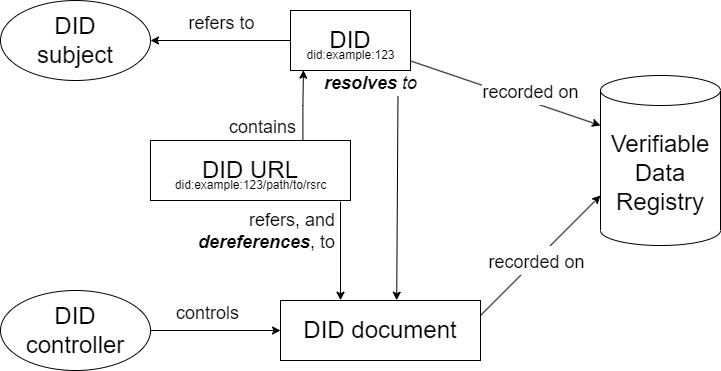
\includegraphics[width=10cm]{./chapters/images/did-overview.png}
    \caption{DID architecture overview and relationships between components \cite{didW3C}.}
    \label{didOverview}
\end{figure}

\subsection{Verifiable Credentials}
Verifiable Credential \cite{vcW3C} provides a standard method to express credentials on the internet in a way that is cryptographically safe, privacy-respecting, and machine-verifiable.
In our daily lives a credential could consist of:
\begin{itemize}
    \item information related to identifying the subject of the credential (for example, a photo, name, or identification number)
    \item information related to the issuing authority (for example, a city government or a university)
    \item information related to the type of credential this is (for example, a passport or a driving license)
    \item information related to specific attributes or properties being asserted by the issuing authority about the subject (for example, nationality, the classes of vehicle entitled to drive, or date of birth)
    \item information related to constraints on the credential (such as expiration date, or terms of use). 
\end{itemize}

In verifiable credentials, the inclusion of digital signatures makes them more trustworthy and more tamper-evident against physical credentials allowing third-party verified machine-readable personal information usable on the Web for receiving services and benefits as in the physical world \cite{vcW3C}.

\subsubsection*{Overview}

Distinct actors can be identified in the verifiable credentials ecosystem, which defines the roles and the relationships between them. The separation of roles allows the standardization of interfaces and protocols. In detail the existing entities that determine the \textit{trust triangle} \cite{trustOverIP} are: 

\begin{itemize}
    \item \textit{holder}: his role is to request, possess or use verifiable credentials. Example holders include students, employees, and customers.
    \item \textit{issuer}: his role is to create a verifiable credential and provide that to a holder by asserting claims about one or more subjects. For example, an issuer is a government. 
    \item \textit{verifier}: his role is to process verifiable credentials provided by holders. Example verifiers are whoever provides a service. 
\end{itemize}

\begin{figure}[h!]
    \centering
    \includesvg[inkscapelatex=false, scale=0.70]{./chapters/images/vc-ecosystem.svg}
    \caption{The roles and information flows of Verifiable Credential \cite{vcW3C}.}
    \label{vcEcosystem}
\end{figure}

Verifiable credentials and verifiable presentations can be represented in JSON \cite{json-rfc3986} or JSON-LD \cite{json-ld} format as can be seen in listings \ref{vcExample} and \ref{vpExample}. 

\begin{lstlisting}[caption={A simple example of a verifiable credential \cite{vcW3C}.},captionpos=b,style=json, label={vcExample},breaklines=true,frame=single]
{
    "@context": [
        "https://www.w3.org/2018/credentials/v1",
        "https://www.w3.org/2018/credentials/examples/v1"
    ],
    "id": "http://example.edu/credentials/1872",
    "type": ["VerifiableCredential", "AlumniCredential"],
    "issuer": "https://example.edu/issuers/565049",
    "issuanceDate": "2010-01-01T19:23:24Z",
    "credentialSubject": {
        "id": "did:example:ebfeb1f712ebc6f1c276e12ec21",
        "alumniOf": {
            "id": "did:example:c276e12ec21ebfeb1f712ebc6f1",
            "name": [{
                "value": "Example University",
                "lang": "en"
            }]
        }
    },    
    "proof": {
        "type": "RsaSignature2018",
        "created": "2017-06-18T21:19:10Z",
        "proofPurpose": "assertionMethod",
        "verificationMethod": "https://example.edu/issuers/565049#key-1",
        "proofValue": "eyJhbGciOiJSUzI1NiIsImI2NCI6ZmFsc2UsI..."
        }
}
\end{lstlisting}

\begin{lstlisting}[caption={A simple example of a verifiable presentation \cite{vcW3C}.},captionpos=b,style=json, label={vpExample},breaklines=true,frame=single]
    {
        "@context": [
          "https://www.w3.org/2018/credentials/v1",
          "https://www.w3.org/2018/credentials/examples/v1"
        ],
        "type": "VerifiablePresentation",
        "verifiableCredential": [{
            ...
        }],
        "proof": {
          "type": "RsaSignature2018",
          "created": "2018-09-14T21:19:10Z",
          "proofPurpose": "authentication",
          "verificationMethod": "did:example:ebfeb1f712ebc6f1c276e12ec21#keys-1",
          "challenge": "1f44d55f-f161-4938-a659-f8026467f126",
          "domain": "4jt78h47fh47",
          "proofValue": "Qy72IFLN25DYuNzVBAh4vGHSrQyHUGlc..."
        }
      }   
\end{lstlisting}

\subsection{Distributed Ledgers Technologies}

Distributed Ledger Technology (DLT)  is a new paradigm for collecting and sharing information between people. A distributed ledger is a database that is spread across several nodes or computing devices. An exact copy of the ledger is replicated and stored on each node. The revolutionary aspect of distributed ledger technology is that no single administrator or central authority is responsible for maintaining the ledger. Each network's participant node keeps its state updated by constructing and recording updates to the ledger independently. The nodes then vote on these adjustments to ensure that the majority agrees with the conclusion reached. This voting and agreement on the state of the ledger is called consensus and is conducted automatically via a consensus algorithm \cite{dlt-intro-1}. 
The following criteria can be used to categorize DLTs: data structures, consensus algorithms, permissions, mining accessibility and so on. The main data structure types are blockchains and Directed Acyclic Graphs (DAGs). Although blockchains are the most popular and well-known DLT type,  DLTs based on Directed Acyclic Graph (DAG) data structures are becoming more popular because they reduce transaction data size and transaction fees, and increase transaction speeds \cite{dlt-intro-2}.

An Example of DAG DLT is the \textit{tangle} of IOTA \cite{popov2018tangle}, a cryptocurrency for the Internet-of-Things (IoT) industry.

\begin{figure}[h!]
    \centering
    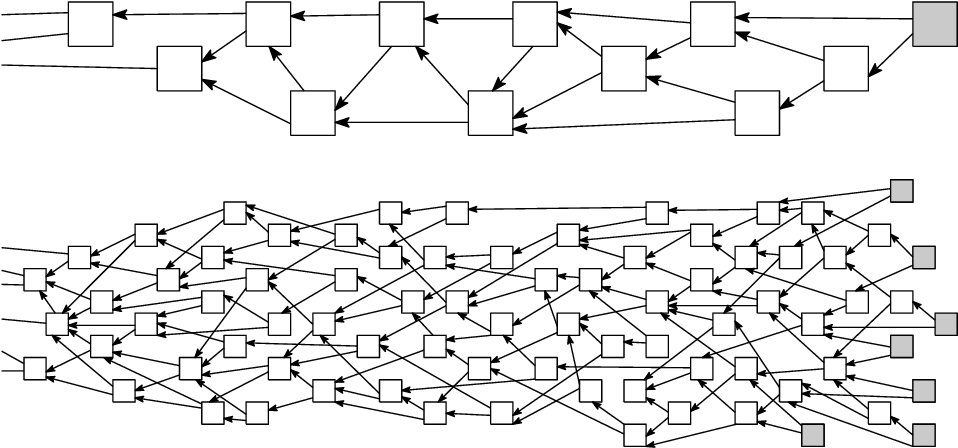
\includegraphics[width=10cm]{./chapters/images/tangle.png}
    \caption{Visualizations of the IOTA tangle \cite{popov2018tangle}.}
    \label{tangleFigure}
\end{figure}


\section{Keystone Enclave}
Device manufacturers are now taking security concerns more seriously than they previously did as a result of the rise in popularity of networked devices in recent years.
To adequately address these challenges, a specification has been developed that defines a way to ensure the integrity and confidentiality of sensitive data in the device that implements the specification.
\cite{IntroTEE}
\subsection{Trusted Execution Environment}
A Trusted Execution Environment (TEE) is a safe area within a CPU. It runs in an isolated environment and in parallel with the operating system.
It ensures that the confidentiality and integrity of the code and data loaded in the TEE are preserved. 
Trusted applications running on TEE have access to the full capabilities of a device's main processor and memory, while hardware isolation shields these components from user-installed apps running in the main operating system. The various included trusted applications are protected from one another by software and cryptographic isolations within the TEE.
\cite{IntroTEE}
%aggiungere definizione di enclave, tcb?
The two most common TEE implementations at the moment are ARM TrustZone and Intel SGX. All these TEEs make design decisions based on either the target applications or threat models and these choices are fixed since they are strictly hardware related. They were not designed to have flexibility or extensibility for enclave developers.  If the hardware changes or has a new feature, the enclave developer has to redesign the TEE.
All TEE platforms aim to reduce the enclave's TCB, yet they have managed to achieve different degrees of success. Additionally, closed-source hardware and microcode implementations make it impossible for a third party to evaluate the security of TEEs.



\textbf{Customizable TEE} is the solution to these problems. It has been designed to be flexible, configurable and to have a small TCB. It has been developed with clear abstractions and a modular programming model which simplifies for others to extend and add features to the TEE. A customizable TEE is Keystone.
\cite{lee2020keystone} 
\subsection{Keystone overview}
Keystone \cite{lee2020keystone} is an open-source framework for creating RISC-V hardware-based Trusted Execution Environments (TEEs) that are adaptable for use on a variety of platforms. Keystone offers security primitives that can be joined together via the software framework rather than creating a single instance of TEE hardware. The TEE can be modified by the creator of the enclave and the platform provider to suit their threat models or platform configurations. The Keystone project offers a general and formally proven interface for a variety of devices to create an open standard for TEEs. Every piece of hardware could, in our opinion, have a secure TEE at practically no extra cost.

\begin{figure}[h!]
    \centering
    \includesvg[inkscapelatex=false, scale=0.40]{./chapters/images/TEE-keystone-vs-x86.svg}
    \caption{architecture differences between x86 and keystone}
    \label{keystone-vs-x86}
\end{figure}
\subsubsection{Security Monitor}
\subsubsection{Runtime}

\chapter{Design and Implementation}

%!TEX encoding = IsoLatin
%!TEX main = ../../main.tex

\section{Self-Sovereign-Identity as a Service}
\subsection{Use case analysis}

\subsection{Design}
grafico generale delle operazioni
\subsection{Implementation}


\chapter{Setup, test and result analysis}

%!TEX encoding = IsoLatin
%!TEX main = ../../main.tex

%\section{Self-Sovereign-Identity as a Service}
The idea of a Self-Sovereign-Identity as a Service is to support a constrained device to create and manage its self-sovereign-identity. Since IoT devices cannot run natively the complete SSI stack there is a need to design and develop an edge device capable of providing such an identity to constraint devices as a service.  Such a solution has the advantage of increasing the number of devices that can interact in such a secure digital ecosystem.

\section{Use case analysis}
The first step is to analyse and identify critical cryptographic operations involved in self-sovereign-identity management.The examples in figures \ref{usecase-did}, \ref{usecase-issuer} and \ref{usecase-verifier} illustrate in an high-level way how to create and use verifiable credentials. 
\begin{figure}[!h]
    \centering
    \includesvg[inkscapelatex=false, scale=0.80]{./chapters/images/use-case-did_creation.svg}
    \caption{Creation of a DID}
    \label{usecase-did}
\end{figure}

\subsection{Creation of a DID}
Independently from the chosen registry when a holder creates a DID, he uniquely binds cryptographic proofs with the DID identifier, typically using public-private key pairs, so he will need to generate them before generating the DID document. The order of operations can be seen in figure \ref{usecase-did}. 
\subsection{Verifiable Credential Issuance}
\begin{figure}[!h]
    \centering
    \includesvg[inkscapelatex=false, scale=0.80]{./chapters/images/use-case-credential_creation.svg}
    \caption{Issuance - verifiable credential creation}
    \label{usecase-issuer}
\end{figure}
Next, a holder can get a verifiable credential from an issuer, that will verify the identity in some way, by examining the provided documentation, if the requirements are satisfied the issuer will generate a verifiable credential by linking her identity information to DID. The holder receiving the verifiable credential will verify its validity and save it in his personal credential repository. All of this is shown in figure \ref{usecase-issuer}. 
\subsection{Verifiable Credential Verification}
\begin{figure}[!h]
    \centering
    \includesvg[inkscapelatex=false, scale=0.80]{./chapters/images/use-case-credential_usage.svg}
    \caption{Verification - verifiable credential usage}
    \label{usecase-verifier}
\end{figure}

Moreover, as can be seen in figure \ref{usecase-verifier}, once a holder has a DID and a verifiable credential, he can use them to access a service to a verifier. The holder will use the DID to prove to the requesting party that it is the controller of that DID through some sort of challenge-response. Then the holder, starting from one or more verifiable credentials will create a verifiable presentation. If possible it is recommended to the holder use selective disclosure, presenting proofs of claims without revealing the entire verifiable credential. Once created the verifiable presentation the holder can send it to the verifier and he will check its validity and authorize the holder if everything is fine.  
\section{Performance analysis}
After analysing the different use cases, as highlighted in figures \ref{usecase-did}, \ref{usecase-issuer} and \ref{usecase-verifier}, the cryptographic operations that could be  critical for a constrained device are:
\begin{itemize}
    \item keys generation
    \item signature generation and verification
    \item proof generation and verification
\end{itemize}

To understand how much critical these operations are on a constrained device it is necessary to analyse the differences between a non-constrained one by getting their execution times and comparing the result. 
STM32L4+ Discovery kit IoT node\cite{stm32-board-product} has been used as a constrained device equipped with the \texttt{STM32L4S5 MCU @ 120 MHz}, 2 Mbytes of flash memory and 640 Kbytes of SRAM. While, as a non-constrained device, which has also been called \textit{edge device}, has been used a server with an \texttt{Intel Xeon Silver 4110 CPU @ 2.10GHz}. 

\begin{figure}[h!]
    \centering
    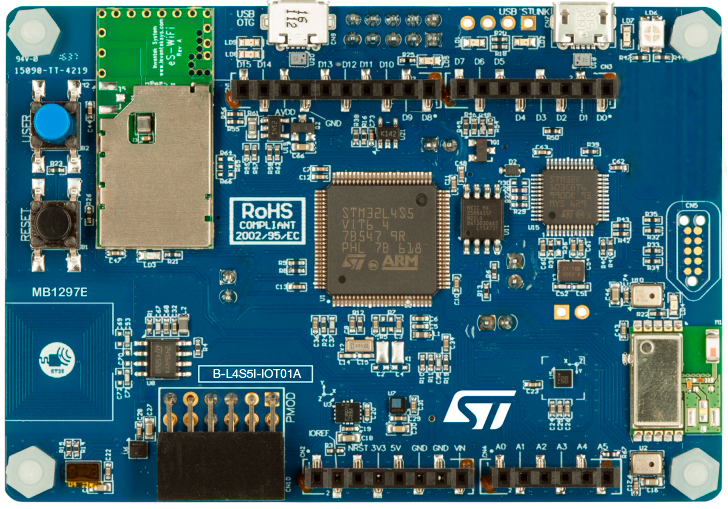
\includegraphics[scale=0.30]{./chapters/images/STM32L4+ Discovery kit IoT node.jpeg}
    \caption{STM32L4+ Discovery kit IoT node\cite{stm32-board-product}.}
    \label{stm-board}
\end{figure}

As a library that implements the operation for key generation and signature (generation and verification), Mbed TLS has been used. \textit{Mbed TLS} is a C library that implements cryptographic primitives, it supports RSA, ECDSA, and other algorithms such as Ed25519. It has a small code footprint which makes it reasonable to use for embedded systems \cite{mbed-tls}. To test if a constrained device could be capable to implement and use some \textit{zero-knowledge proof} mechanisms, it has been decided to use a library which implements the BBS\texttt{+} signature scheme \cite{bbsplus}. BBS\texttt{+} signatures can be used to generate signature proofs of knowledge and selective disclosure zero-knowledge proofs \cite{bbs-rust} and they are implemented on top of BLS12-381 elliptic curve \cite{bls-curve}, which is a curve not supported in Mbed TLS. Since available BBS\texttt{+} libraries are also not supported for STM32L4, it has been decided to take execution times only on the edge device. Then execution times between the ECDSA signature scheme and BBS\texttt{+} signature scheme are comparable since they are been taken on the same architecture and they are both elliptic curve signature schemes.

\section{Results}
It is evident from the table \ref{time-table1} that RSA is usable on constrained devices in real-life applications only if the key generation is precomputed, otherwise is unusable. On the constrained device, RSA signing and verification are faster than ECDSA, but ECDSA provides the same level of security as RSA but it does so while using much shorter key lengths. In applications where it could be useful to generate a keypair on the fly, ECDSA is a must. On the edge device, the ECDSA signing operation is faster than RSA, while the RSA verification process is faster than ECDSA.  It can also be noted that the time difference between the constrained device and the edge device is huge, probably due to the frequency of operation of the MCU and the CPU.

\begin{table}[!h]
    \centering
    \begin{tabular}{| l || r | r | r |}
        \hline      
        \textbf{Operation} & \textbf{constrained device}$^\star$ & \textbf{edge device}$^\star$ \\ [0.5ex] 
        \hline \hline 
        EC-p256-keygen                  & 318 ms  & 0.5 ms \\
        \hline
        ECDSA-p256-SHA256-sign          & 1\,503 ms & 0.6 ms \\
        \hline
        ECDSA-p256-SHA256-ver           & 6\,031 ms & 2.0 ms \\
        \hline \hline
        RSA2048-keygen                  & 622\,749 ms  & 186  ms \\
        \hline
        RSA2048-SHA256-sign          & 1\,305 ms & 3.60 ms \\
        \hline
        RSA2048-SHA256-ver           & 331 ms & 0.07  ms \\
        \hline
    \end{tabular}\\
    \footnotesize $^\star$mbedTLS library
    \caption{Execution time comparison between constrained and non-constrained devices}
    \label{time-table1}
\end{table}

Furthermore, in table \ref{time-table2} ECDSA signatures and BBS\texttt{+} signatures are compared on the same CPU architecture. The obtained results are that BBS\texttt{+} signature scheme is much slower than the ECDSA one, even if they are both elliptic curve based. The order of magnitude of the percentage increase is 3, which is a significant difference. 
   
\begin{table}[!h]
    \centering
    \begin{tabular}{| l || r | r | r|}
        \hline 
        \textbf{Operation} & \textbf{ECDSA}$^\star$ & \textbf{BBS\texttt{+}}$^\star$$^\dagger$ & \textbf{\% increase} \\ [0.5ex] 
        \hline  \hline 
        keygen   & 0.2   ms      & 39 ms   &\texttt{+}7\,800\\
        \hline
        sign     & 0.6   ms      & 27  ms   &\texttt{+}4\,500\\
        \hline
        verify   & 2.0  ms         & 166 ms   &\texttt{+}8\,300\\
        \hline
    \end{tabular}
    \\
    \footnotesize $^\star$Xeon 2.10GHz \enspace\enspace $^\dagger$Rust bbs library
    \caption{Execution time comparison between ECDSA and BBS\texttt{+}}
    \label{time-table2}
\end{table}

\section{Design and implementation choices}
The obtained results suggest that a constrained device cannot use the BBS\texttt{+} signature scheme in real-world applications, since it can be supposed that execution times will be considerably high. In the Self-sovereign Identity as a Service (SSIaaS) paradigm, a new role is defined, called edge. The edge device interacts with a constrained IoT object and provides functionalities to create and support it in identity management, this can be seen in figure \ref{poc-design}. The identified and exposed operations by the edge device are:
\begin{itemize}
    \item key pairs generation
    \item storage of a verifiable credential
    \item generation of a verifiable presentation
\end{itemize}

\subsection{Self-Sovereign-Identity as a Service Ecosystem}

\begin{figure}[!h]
    \centering
    \includesvg[inkscapelatex=false, scale=1]{./chapters/images/poc.svg}
    \caption{Basic components of Self-Sovereign-Identity as a Service}
    \label{poc-design}
\end{figure}

From now on, the focus is on the interaction between the edge device and the IoT-constrained node. The IoT device can request the edge node to generate key pairs that could later use to generate a verifiable presentation. The IoT device can store on the edge node a verifiable credential got from an issuer. If the IoT device what to interact with a verifier, it has to provide a verifiable presentation, which is generated by the edge device starting from the verifiable credential and signing the vc with a keypair previously generated for that specific IoT client. 
Since these are security-critical operations because they handle the identity of the IoT node, it needs the guarantee that the data shared with the edge device and the executed code are protected with respect to confidentiality and integrity. Hence, a TEE has been implemented using the keystone framework.  Figures \ref{manufacturer-provisioning} and \ref{poc-architecture} show the architecture and the preliminary interactions between the IoT device and the edge device, before the constrained device can ask for services. Figures \ref{poc-gen-keys}, \ref{poc-store-vc} and \ref{poc-get-vp} show in a top-level way how the operations have been implemented. 

\subsection{IoT Device Provisioning}

The first step before deploying an IoT device in the network is its provisioning. Provisioning means configuring the IoT device to be ready when joining the network to communicate with and be authenticable by the edge device. In the implemented solution, a trustworthy system administrator provisions the client, i.e., the constrained device, with: 
\begin{itemize}
    \item a key pair (client secret and public keys) used to authenticate itself to the server, i.e., the edge device
    \item expected security monitor and enclave hashes to verify that the edge device is running the expected application in the enclave 
    \item the device public key of the edge device to verify that is running on trusted hardware
\end{itemize} 

\begin{figure}[!h]
    \centering
    \includesvg[inkscapelatex=false, scale=0.7]{./chapters/images/manufacturer.svg}
    \caption{Manufacturer provisions device with expected hashes, keys and signature of the public key}
    \label{manufacturer-provisioning}
\end{figure}

Then, the system administrator signs the public key of the IoT client and saves the signature. The sigature is verifiable with the public key of the system administrator. It proves (trust assumptions) that the device with access to the client's secret belongs to a recognised IoT network group. This client authentication method was chosen because the edge device only needs to retain the system administrator's public key in memory, rather than keeping track of all the clients' public keys in a database to determine whether a client is authorized to access services.

\subsection{Attestation Report and Session Context}
With the use of ed25519 signatures on hashes of the security monitor and enclave content, Keystone supports a basic attestation mechanism, as introduced in section \ref{keystone-components}. Once an enclave has started the execution, it requests the SM to generate a signed enclave report and a signed SM report. The SM Report enclose a hash of the security monitor and the attestation public key, all signed by the device root key. The enclave report consists of a hash of the enclave at initialization and a data block from the enclave of up to 1Kbytes, 
all signed by the attestation public key. A verifier, in this case, the IoT device when provided with the device public key, expected SM hash, and expected enclave hash will verify the signatures of these reports. An example of an attestation report is shown in listing \ref{attestation-report}. \\

\begin{lstlisting}[caption={Example of a attestation report  generated by the enclave},captionpos=b,style=json, label={attestation-report},frame=single]
{
    "enclaveApplication": {
        "hash": "11ff35526c90c469ca6878dc22494703c554db654...",
        "enclaveData": "b07dfd3047fb5213b8af9b76594a06891...",
        "signature": "58ca380c6b4476ed7b27143d92dec14fff2858ffef8ed6ef4..."
    },
    "securityMonitor": {
        "hash": "e51749130b6036fe85b27409a4ea3e1c078fe4dcb76...",
        "publicKey": "cd98f4a28a8523ba8ecd31175aa0e2330b2f46e70...",
        "signature": "e738f4e708f73ffa4a0d3dc2199c9e0ac119bf14b32da33a..."
    },
    "devicePublicKey": "0faad4ff01178583baa588966f7c1ff32564dd17d..."
}
\end{lstlisting}

When designing the demo, the session context has been introduced to authenticate the client on the server side. The session context includes two sections: the stub certificate and the homonym session context. The first one contains the client's public key and the signature of the client's public key, made at the provisioning phase by the system administrator and verifiable with the public root key. The enclosed session context contains a data block, all signed by the client public key. A verifier, in this case, the edge node when provided with the root public key of the system administrator will verify the signatures of this structure. An example of a session context is shown in listing \ref{session-context}. \\

\begin{lstlisting}[caption={Example of a session context generated by the client},captionpos=b,style=json, label={session-context},frame=single]
{
    "sessionContext": {
        "data": "3a2992fe52a2082b26f8009117be53decff68...",
        "dataSignature": "02b0b554aecd929419a6c525ebfde..."
    },
    "stubCertificate": {
        "clientPublicKey": "e95f84f09574d8fe73c0e692905c6c8d...",
        "rootSignature": "a8b20a77877b79ca0d699091f8b303463b..."
    }
}
\end{lstlisting}

In the demo implementation, the data part of the session context and the attestation report are both used for the Diffie-Hellman key exchange protocol so that the two parties can securely compute a shared key for creating a secure encrypted channel. 

\subsection{Demo Architecture}
In the following description, the implemented architecture has been simplified for development reasons. This demo demonstrates how a remote (constrained) device can request computation to be performed on an untrusted server using an enclave. (The demo uses test keys, it is not safe and should not be used in production). The demo architecture consists of:
\begin{itemize}
    \item a server enclave application and an untrusted host application hosted on a RISC-V processor
    \item an IoT client provisioned by the system administrator  
\end{itemize} 

The demo enclave application has essential enclave capabilities (attestation report generation, data sealing, etc.), uses \texttt{libsodium} for establishing a secure channel and exposes three SSI-related services. The untrusted enclave host serves a few functions: starting the enclave, proxying network packets from and to the client and storing sealed data. The remote client establishes a connection with the untrusted host, verifies the enclave report, transmits the session context, and creates a secure channel before being able to communicate with the host to request offloaded computations. 

\begin{figure}[!h]
    \centering
    \includesvg[inkscapelatex=false, scale=0.7]{./chapters/images/Demo architecture3.svg}
    \caption{Demo architecture}
    \label{poc-architecture}
\end{figure}

\subsubsection{Running the demo}

At the start, the client will connect to the enclave and perform the remote attestation. Expected hashes in the attestation report will be used by the trusted client to verify that the enclave is created with the right application and initialized by the known version of the security monitor. If the attestation is successful, the client can send its attestation, also called session context. The server will check the signature validity provided by the client, verifying it with the public key of the system administrator (\texttt{root\_pk}). On the contrary, if the edge device attestation report is invalid, the client will close the connection. (For instance, you could pass a flag when launching the client to ignore the attestation report of the server for testing purposes or during development when changing the enclave application).
Upon exchanging the session context and the attestation report, they establish a secure channel and the enclave-host waits for messages.

\subsection{Offloaded Operations}
Once the edge node and the constrained devices have established a secure channel to communicate, the enclave waits for the client to request service. Once a message is received, the enclave authenticates and decrypts the message. If successful, it processes the message and passes the request to a specific \textit{ocall}, i.e, \texttt{ocall\_wait\_for\_request(...)}, which dispatches the requests proxied by the untrusted host coming from the client. By checking the request type, the enclave understands what service the client has requested. After processing the request, the enclave returns the result through the secure channel.

\subsubsection{Generate public keys}
\begin{figure}[!h]
    \centering
    \includesvg[inkscapelatex=false, scale=0.7]{./chapters/images/poc_gen_keys.svg}
    \caption{Key pairs generation operation (pseudo-code)}
    \label{poc-gen-keys}
\end{figure}
\subsubsection{Store verifiable credential}
\begin{figure}[!h]
    \centering
    \includesvg[inkscapelatex=false, scale=0.7]{./chapters/images/poc_store_vc.svg}
    \caption{Storage of a verifiable credential operation (pseudo-code)}
    \label{poc-store-vc}
\end{figure}
\subsubsection{Get verifiable presentation}
\begin{figure}[!h]
    \centering
    \includesvg[inkscapelatex=false, scale=0.7]{./chapters/images/poc_get_vp.svg}
    \caption{Generation of a verifiable presentation operation (pseudo-code)}
    \label{poc-get-vp}
\end{figure}



\chapter{Conclusion and future work}

Qui si inseriscono brevi conclusioni sul lavoro svolto, senza ripetere inutilmente il sommario.

Si possono evidenziare i punti di forza e quelli di debolezza, nonch? i possibili sviluppi futuri o attivit? da svolgere per migliorare i risultati.

% bibliografia scritta "a mano"
%% !TEX encoding = IsoLatin

% La bibliografia, da inserirsi solo se ci sono state citazioni.
% In questo caso ricordarsi che bisogna sempre elaborare due volte il file .TEX
% perch� la prima volta viene generata la bibliografia mentre la seconda volta viene inclusa

% NOTA: citare il DOI non � obbligatorio ma MOLTO desiderabile
% NOTE: inserting the DOI is not compulsory bur STRONGLY recommended whenever it exists

\begin{thebibliography}{9} % se ci sono meno di 10 citazioni
%\begin{thebibliography}{99} % se ci sono da 10 a 99 citazioni
%\begin{thebibliography}{999} % se ci sono da 100 a 999 citazioni

% esempio citazione articolo a congresso
% example: reference to a conference paper
\bibitem{psisec}
% autori - authors
I.Enrici, M.Ancilli, A.Lioy,
% titolo articolo - article title
``A psychological approach to information technology security'',
% nome del congresso - conference name
HSI-2010: 3rd Int. Conf. on Human System Interactions,
% luogo (stato) e data del congresso
% town (country) and date of the conference
Rzesz�w (Poland), May 13-15, 2010,
% pagine dell'articolo - article pages
pp.\ 459-466,
% DOI
\doi{10.1109/HSI.2010.5514528}

% esempio citazione articolo su rivista
% example: reference to a journal/magazine article
\bibitem{tpa}
% autori- authors
G.Cabiddu, E.Cesena, R.Sassu, D.Vernizzi, G.Ramunno, A.Lioy,
% titolo dell'articolo -  article title
``Trusted Platform Agent'',
% nome della rivista - name of the journal
IEEE Software,
% volume e numero della rivista (alcune riviste non ce l'hanno)
% volume and issue number (some journals don't have it)
Vol.\ 28, No.\ 2,
% mese e anno di pubblicazione della rivista
% month and year when paper appeared in the journal
March-April 2011,
% pagine dell'articolo  - article pages
pp.\ 35-41,
% DOI
\doi{10.1109/MS.2010.160}


% esempio citazione capitolo di un libro fatto come collezione di contributi da autori diversi
% example: reference to the chapter of a book which is a collection of chapters from different authors
\bibitem{tc}
A.Lioy, G.Ramunno, % autori del capitolo
``Trusted Computing'' % titolo del capitolo
nel libro % in the book
``Handbook of Information and Communication Security'' % titolo del libro
a cura di % edited by
P.Stavroulakis, M.Stamp, % nomi dei curatori
Springer, % nome editore
2010, % anno di pubblicazione
pp.\ 697-717, % pagine del capitolo
\doi{10.1007/978-3-642-04117-4_32}

% esempio citazione pagina web di un progetto
% example: reference to the web page pof a project
\bibitem{openssl}
% nome del progetto - name of the project
The OpenSSL project,
 % URI della pagina web - URI of the web page
\url{http://www.openssl.org/}

% esempio citazione RFC
% example: reference to a RFC
\bibitem{tls12}
T.Dierks, E.Rescorla,
``The Transport Layer Security (TLS) Protocol Version 1.2'',
\rfc{5246}, August 2008,
\doi{10.17487/RFC5246}

% esempio: citazione libro
% example: reference to a book
\bibitem{seceng}
Ross J. Anderson,
``Security engineering'',
Wiley, 2008,
ISBN: 978-0-470-06852-6

\end{thebibliography}


% se la bibliografia ? stata scritta (usando Bibtex) nel file biblio.bib allora commentare la riga precedente e scommentare le due righe seguenti
\bibliographystyle{other/torsec}
\bibliography{other/biblio}

\appendix
\chapter{User Manual}
%!TEX encoding = IsoLatin
%!TEX main = ../../main.tex


\chapter{Developer manual}
%!TEX encoding = IsoLatin
%!TEX main = ../../main.tex

\section{Developer manual}
\subsection{Constrained and edge device comparison}
\subsubsection{Test MbedTLS library}
{\color{red} ToDo: spiegare come il progetto e' organizzato e file/funzioni rilevanti}
\subsubsection{Test BBS\texttt{+} signatures scheme}
For this subproject the most relevant files are:
\begin{itemize}
  \item \texttt{Cargo.toml} where dependencies are added, such as  
  \texttt{bbs} and \texttt{rand}. 
  \item \texttt{main.rs} where tests for BBS\texttt{+} key generation, signature and verification are defined. 
  \begin{itemize} 
    \item \texttt{fn key\_gen\_test(iterations: usize)}
    \item \texttt{fn simple\_sign\_ver\_test(iterations: usize)}
    % \item \texttt{fn pok\_sign\_ver\_test(iterations: usize)}
  \end{itemize}
\end{itemize}
And the code is very simple, it launches the test for key generation and the test for signature and verification, operations are executed \texttt{iterations} times and the average is displayed on the output video. 
\begin{lstlisting}[frame=single]
fn main() {
  let iterations: usize = 100;
  key_gen_test(iterations);
  simple_sign_ver_test(iterations);
}
\end{lstlisting}

\subsection{Proof of concept}
\subsection*{Guide to Keystone Components}
The Keystone repository consists of several sub-components such as gitmodules or directories. This is a brief overview of them.
\begin{lstlisting}[frame=single]
+ keystone/
|-- patches/
|  # required patches for submodules
|-- bootrom/
|  # Keystone bootROM for QEMU virt board, including trusted boot chain.
|-- buildroot/
|  # Linux buildroot. Builds a minimal working Linux image for our test platforms.
|-- docs/
|  # Contains read-the-docs formatted and hosted documentation, such as this article.
|-- riscv-gnu-toolchain/
|  # Unmodified toolchain for building riscv targets. Required to build all other components.
|-- linux-keystone-driver/
|  # A loadable kernel module for Keystone enclave.
|-- linux/
|  # Linux kernel
|-- sm/
|  # OpenSBI firmware + Keystone security monitor
|-- qemu/
|  # QEMU
+-- sdk/
    # Tools, libraries, and example apps for building enclaves on Keystone        
\end{lstlisting}

\subsection*{Guide to Keystone Demo Proof of concept}
The designed solution has been developed starting from the officially \texttt{kestone-demo} repository available at this link: \url{https://github.com/keystone-enclave/keystone-demo}. The demo uses test keys and is not safe for production use.
\begin{lstlisting}[frame=single]
  + keystone-demo-poc/
  |-- docs/
  |  # Contains read-the-docs formatted and hosted documentation, such as this article.
  |-- include/
  |  # Contains shared files between eapp and client
  |-- scripts/
  |  # Contains a script for performing the attestation of sm and eapp
  |-- server_eapp/
  |  # small enclave server that is capable of remote attestation, secure channel creation, and performing a simple word-counting computation securely
  |-- sodium_patches/
  |  # Contains patch for libsodium that will run in the server eapp
  +-- trusted_client/
     # simple remote client that connects to the host, validates the enclave report, constructs a secure channel, and then can send messages to the host for computation.       
  \end{lstlisting}

\subsection*{Relevant files of the demo}
Below are explained relevant files that change from the official \texttt{kestone-demo} repository.

\subsubsection{include/eh\_shared.h}
This file is shared between the enclave and the untrusted host. It defines the following data structure for exchanging sealed (encrypted) data between the enclave and the untrusted host. 

\begin{lstlisting}[language=C,frame=single]
typedef struct stored_data_t{
  unsigned short file_type;
  unsigned char client_pk[crypto_kx_PUBLICKEYBYTES];
  size_t c_len;  
  unsigned char content[]; // Flexible member
} stored_data_t;      
\end{lstlisting}

\subsubsection{include/messages.h}
This file is shared between the client and the enclave and it defines the messages (request amd response) they exchange. 
\begin{lstlisting}[language=C,frame=single]
typedef struct request_message_t{
  unsigned short request_type;
  unsigned char secret[SECRET_LEN];
  size_t len;
  unsigned char payload[]; // Flexible member
} request_message_t;

typedef struct response_message_t{
  unsigned short response_type;
  size_t len;
  unsigned char payload[]; // Flexible member
} response_message_t;
\end{lstlisting}


\subsubsection{include/session\_context.c and include/session\_context.h}
The session context is the structure that the client provides to the enclave to prove that is built by a trusted manufacturer. With the function \texttt{session\_context\_from\_buffer} the session context is extracted from the received buffer. 
\begin{lstlisting}[language=C,frame=single]
struct session_context_t {
  unsigned char  dh_public_key[PUBLIC_KEY_SIZE];
  unsigned char  challenge[CHALLENGE_SIZE];
  unsigned char  data_signature[SIGNATURE_SIZE];
  
  unsigned char  client_public_key[PUBLIC_KEY_SIZE];
  unsigned char  root_signature_of_client_pk[SIGNATURE_SIZE];
};

void session_context_from_buffer(struct session_context_t* session_context, unsigned char* buffer);
\end{lstlisting}

\noindent
\texttt{int session\_context\_verify( ... );}\\
\textit{Input}:
\begin{itemize}[noitemsep,nolistsep]
  \item \texttt{struct session\_context\_t session\_context}, the session context to verify
  \item \texttt{unsigned char* challange}, the challenge that the server has sent to the client
  \item \texttt{const unsigned char* root\_public\_key}, the public key of the manufacturer
\end{itemize}
\textit{Output}: an \texttt{int} value, 1 if it is a valid session context, 0 if not.

\subsubsection{server\_eapp/service.c and server\_eapp/service.h}
The file \texttt{service.h} just exposes the function that processes the request received by the client.  
\begin{lstlisting}[language=C,frame=single]
response_message_t *process_request(request_message_t *request, size_t *pt_finalsize) {

  struct sealing_key sealing_material;
  int ret = 0;

  /* Derive the sealing key */
  ret = get_sealing_key(&sealing_material, sizeof(sealing_material),
                        (void *)request->secret, SECRET_LEN);

  if (ret) {
    ocall_print_buffer("Sealing key derivation failed!\n");
    EAPP_RETURN(-1);
  }

  switch (request->request_type) {
  case SERVICE_GEN_KEYS:
    return generate_public_keys(pt_finalsize, sealing_material, (int)*request->payload - '0');
    break;
  case SERVICE_STORE_VC:
    return store_verifiable_credential(pt_finalsize, sealing_material, request->payload, request->len);
    break;
  case SERVICE_GET_VP:
    return get_verifiable_presentation(pt_finalsize, sealing_material, request->payload, request->len);
    break;
  }
  return NULL;
}
\end{lstlisting}
{\color{red} ToDo: esplicitare cosa indicano i valori in input e qual e' l'output}\\
\noindent
\texttt{void store\_data ( ... );}\\
\textit{Input}:
\begin{itemize}[noitemsep,nolistsep]
  \item \texttt{unsigned char* buffer}
  \item \texttt{size\_t len}
  \item \texttt{unsigned short file\_type}
\end{itemize}
\textit{Output}: 

\noindent
\texttt{void seal\_data\_and\_sign ( ... );}\\
\textit{Input}:
\begin{itemize}[noitemsep,nolistsep]
  \item \texttt{unsigned char* data}
  \item \texttt{size\_t data\_len}
  \item \texttt{unsigned char** ciphertext}
  \item \texttt{size\_t* ciphertext\_len}
  \item \texttt{unsigned char** sign}
  \item \texttt{size\_t* sign\_len}
  \item \texttt{struct sealing\_key sealing\_material}
\end{itemize}
\textit{Output}: 


\noindent
\texttt{response\_message\_t* build\_response ( ... );}\\
\textit{Input}:
\begin{itemize}[noitemsep,nolistsep]
\item \texttt{size\_t* pt\_finalsize}
\item \texttt{unsigned char *buffer}
\item \texttt{size\_t len}
\end{itemize}
\textit{Output}: 


\noindent
\texttt{response\_message\_t* generate\_public\_keys ( ... );}\\
\textit{Input}:
\begin{itemize}[noitemsep,nolistsep]
\item \texttt{size\_t* pt\_finalsize}
\item \texttt{struct sealing\_key sealing\_material}
\item \texttt{int key\_type}
\end{itemize}
\textit{Output}: 

\noindent
\texttt{response\_message\_t* store\_verifiable\_credential ( ... );
}\\
\textit{Input}:
\begin{itemize}[noitemsep,nolistsep]
  \item \texttt{size\_t* pt\_finalsize}
  \item \texttt{struct sealing\_key sealing\_material}
  \item \texttt{unsigned char* vc}
  \item \texttt{size\_t vc\_len}
\end{itemize}
\textit{Output}: 

\noindent
\texttt{response\_message\_t* get\_verifiable\_presentation ( ... );
}\\
\textit{Input}:
\begin{itemize}[noitemsep,nolistsep]
  \item \texttt{size\_t* pt\_finalsize}
  \item \texttt{struct sealing\_key sealing\_material}
  \item \texttt{unsigned char* nonce}
  \item \texttt{size\_t nonce\_len}
\end{itemize}
\textit{Output}: 

\subsubsection{server\_eapp/server\_eapp.c}
In this file the important functions to mention are:
\begin{itemize}
  %\item \texttt{void validate\_session\_context(void* buffer, unsigned char* challange)}
  \item \texttt{void attest\_and\_establish\_channel()}
  \item \texttt{void handle\_requests()}
\end{itemize}
{\color{red} ToDo: spiegare queste funzioni}\\

\subsubsection{trusted\_client/trusted\_client.c and trusted\_client/trusted\_client.h}
In this file the important functions to mention are:
\begin{itemize}[noitemsep,nolistsep]
  % \item \texttt{}
  \item \texttt{void gen\_session\_context(byte* buffer)} 
  \begin{itemize}[noitemsep]
    \item \textit{Input:}
    \item \textit{Output:}
  \end{itemize}

  \item \texttt{request\_message\_t* generate\_message(char* buffer, size\_t buffer\_len, size\_t* finalsize)}
  \begin{itemize}[noitemsep]
    \item \textit{Input:}
    \item \textit{Output:}
  \end{itemize}
  \item \texttt{request\_message\_t* generate\_exit\_message(size\_t* finalsize)}
  \begin{itemize}[noitemsep]
    \item \textit{Input:}
    \item \textit{Output:}
  \end{itemize}
\end{itemize}
% \begin{lstlisting}[language=C,frame=single]
   
% \end{lstlisting}

% \noindent
% \texttt{}\\
% \textit{Input}:\setlist{nolistsep}
% \begin{itemize}[noitemsep]
%   \item 
% \end{itemize}
% \textit{Output}: 

  
\end{document}
